% !TEX root = ../main.tex
\renewcommand{\localPath}{intro}

\setcounter{chapter}{-1}
\chapter{Introduction}

Objectif de la thèse

Plasma, contexte physique

Modèles

Méthodes numériques

Rappel des objectifs et plan

Plan :
\begin{itemize}
  \item[chap 1 :] schémas expo-Lawson pour le cinétique
  \item[chap 2-3 :] cadre général (6D) modèle hybride
\end{itemize}

% section intro
% !TEX root = ../chap3.tex

\section{Introduction}

L'objectif de ce chapitre est d'étendre les stratégies développées pour la résolution d'un modèle hybride linéarisé, présentées dans le chapitre~\ref{chap2}, au cas $1dz-3dv$ permettant de prendre en compte, entre autre, les effets du champ magnétique sur la dynamtique des particules. Nous étudierons dans ce chapitre un modèle hybride, ce qui suppose que la distribution de particules est composée de deux populations, une première ayant une vitesse thermique faible, et considérée comme \emph{froide}, dont on approximera la dynamique comme celle d'un fluide ; une seconde population ayant une vitesse thermique plus élevée, considérée comme \emph{chaude}, mais contrairement au chapitre~\ref{chap2}, celle-ci n'a pas besoin d'être distribuée selon une bi-maxwellienne. Ce type de modèle peut être utilisé pour modéliser des particules d'un plasma dans un tokamak, ou des particules du vent solaire interagissant avec la magnétosphère terrestre. Dans ces contextes les particules se déplacent de manière hélicoïdale selon les lignes du champ extérieur $\vb{B}_0 = (0,0,B_0)^\top$, et seul le déplacement dans cette direction sera étudié ici, ce qui explique le nom de la seule variable d'espace considérée : $z$. Pour le déplacement hélicoïdale complet \Josselin{il faudrait ajouter ici une référence que je n'ai pas car je ne connais pas trop ces modèles, de mémoire c'est ce que faisait Xiaofei}.

La prise en compte des effets du champ magnétique dans le modèle nous mène à considérer un système à 7 inconnues $(j_{c,x},j_{c,y},B_x,B_y,E_x,E_y,f_h)$, ce qui induit un coût de calcul bien plus important avec les méthodes eulériennes que nous étudions. Pour diminuer ce coût de calcul nous souhaitons diminuer le nombre d'itérations tout en assurant la stabilité des méthodes considérées ; cela se fait en augmentant le pas de temps $\Delta t$ et en estimant les contraintes de stabilité. L'utilisation de méthodes d'ordre élevés en temps, en espace et en vitesse, permet de réduire l'erreur, capturer la dynamique non-linéaire du système, avec peu de points de discrétisation.

Nous souhaitons dans ce chapitre comparer deux méthodes d'ordre élevé en temps et dans l'espace des phrases, sur un cas à 4 dimensions, plus proches d'applications physiques, il s'agit d'une généralisation des deux stratégies développées dans le chapitre~\ref{chap2}, une méthode de \emph{splitting} et une méthode de Lawson. La contrainte du nombre de dimensions ne permet pas de raffiner le maillage\footnote{Pour une discrétisation de $128$ points par direction, la grille contient $128^4$ points, soit, représentées avec des réels à virgule flottante à double précision (64 bits), un espace mémoire de 2Go pour la seule variable $f_h$ ; une méthode de Lawson d'ordre 4 nécessite la sauvegarde des étages intermédiaires, donc $4\times 2\textrm{Go}$ minimum. L'utilisation de transformées de Fourier impose de travailler avec des nombres complexes, ce qui nécessite de doubler l'utilisation mémoire pour la même précision.}, ce qui ne permet pas l'accès à une solution de référence, nous devrons nous contenter de regarder les invariants (comme l'énergie totale), et de comparer les résultats aux taux d'instabilités fournis par les relations de dispersion.

Pour résoudre les problèmes que pose ce problème nous présenterons tout d'abord le modèle hybride $1dz-3dv$, puis nous détaillerons les schémas numériques que nous considérons. La méthode de \emph{splitting} hamiltonien contient 7 étapes, rendant de fait l'ordre élevé (méthode de Suzuki) trop coûteux pour approfondir son étude, nous nous concentrerons donc sur des méthodes de \emph{splitting} d'ordre plus faible. Pour la méthode de Lawson, il est envisageable d'effectuer un filtrage du terme induit pas le champ magnétique externe $\vb{B}_0$, permettant d'augmenter le pas de temps stabilisant la méthode. La partie linéaire du système introduit une matrice dont il n'est pas possible de calculer exactement son exponentielle, pourtant nécessaire pour la mise en œuvre d'une méthode de Lawson perforante. Nous étudierons un premier cas où nous ne profitons pas pleinement de toute la partie linéaire du système, introduisant ainsi une condition de stabilité ; puis nous proposerons une méthode permettant, à l'aide de méthodes approchées comme la troncature de la série de Taylor ou les approximants de Padé, de calculer une approximation de l'exponentielle de toute la partie linéaire, permettant ainsi de se soustraire à une condition de stabilité. \Josselin{Mettre les références vers les sections.}

% section modélisation
% !TEX root = ../chap3.tex

\section{Présentation du modèle}

\begin{align}
  \label{eq:VHM:jx}
  &\pdv{j_{c,x}}{t} = \Omega_{pe}^2 { E}_x - { j}_{c,y}B_0,\\
  \label{eq:VHM:jy}
  &\pdv{j_{c,y}}{t} = \Omega_{pe}^2 { E}_y + { j}_{c,x}B_0,\\
  \label{eq:VHM:Bx}
  &\pdv{B_{x  }}{t} = \partial_z E_y,\\
  \label{eq:VHM:By}
  &\pdv{B_{y  }}{t} = -\partial_z E_x,\\
  \label{eq:VHM:Ex}
  &\pdv{E_{x  }}{t} =-\partial_z B_y - {j}_{c,x} + \int v_x f_h \dd{\vb{v}},\\
  \label{eq:VHM:Ey}
  &\pdv{E_{y  }}{t} =\partial_z B_x - {j}_{c,y} + \int v_y f_h \dd{\vb{v}}, \\
  \label{eq:VHM:fh}
  &\pdv{f_{h  }}{t} +  v_z\partial_z f_h - \left(E_x + v_y B_0 - v_zB_y\right)\partial_{v_x} f_h\\
  &\hspace{2cm}- \left(E_y - v_x B_0 + v_z B_x\right)\partial_{v_y} f_h- \left(v_x B_y- v_y B_x\right)\partial_{v_z} f_h = 0.\nonumber
\end{align}
Cela nous permet de définir l'hamiltonien :
\begin{equation}
  \mathcal{H} = {}
      \underbrace{\frac{1}{2}\int_{\mathbb{R}}(E_x^2+E_y^2) \dd{z}}_{\mathcal{H}_E}
    + \underbrace{\frac{1}{2}\int_{\mathbb{R}}(B_x^2+B_y^2) \dd{z}}_{\mathcal{H}_B}
    + \underbrace{\frac{1}{2}\int_{\mathbb{R}}\frac{1}{\Omega_{pe}^2}(j_{c,x}^2+j_{c,y}^2) \dd{z}}_{\mathcal{H}_{j_c}}
    + \underbrace{\frac{1}{2}\int_{\mathbb{R}}\int_{\mathbb{R}^2}|\vb{v}|^2 f_h \dd{\vb{v}}\dd{z}}_{\mathcal{H}_{f_h}}
  \label{eq:ham1dz3dv}
\end{equation}

On définit le crouchet suivant, définit pour deux fonctionnelles $\mathcal{F}$ et $\mathcal{G}$ :
\begin{equation}
  \begin{aligned}
    \{ \mathcal{F},\mathcal{G} \}[ j_{c,x}, j_{c,y}, B_x, B_y, E_x, E_y, f_h] &=
                       \int_{\mathbb{R}}\int_{\mathbb{R}^3} f_h \left( \partial_z\fdv{\mathcal{F}}{f_h}\partial_{v_z}\fdv{\mathcal{G}}{f_h} - \partial_{v_z}\fdv{\mathcal{F}}{f_h}\partial_z\fdv{\mathcal{G}}{f_h} \right) \dd{\vb{v}}\dd{z} \\
      &\hspace{-4cm} + \int_{\mathbb{R}}\int_{\mathbb{R}^3} f_h \left(
            \partial_{v_x}\fdv{\mathcal{F}}{f_h}\fdv{\mathcal{G}}{E_x} + \partial_{v_y}\fdv{\mathcal{F}}{f_h}\fdv{\mathcal{G}}{E_y}
          - \partial_{v_x}\fdv{\mathcal{G}}{f_h}\fdv{\mathcal{F}}{E_x} - \partial_{v_y}\fdv{\mathcal{G}}{f_h}\fdv{\mathcal{F}}{E_y}
          \right) \dd{\vb{v}}\dd{z} \\
      &\hspace{-4cm} + \int_{\mathbb{R}}\int_{\mathbb{R}^3} f_h(\vb{B}+\vb{B}_0)\cdot\left( \nabla_{\vb{v}}\fdv{\mathcal{F}}{f_h}\times\nabla_{\vb{v}}\fdv{\mathcal{G}}{f_h} \right) \dd{\vb{v}}\dd{z} \\
      &\hspace{-4cm} + \int_{\mathbb{R}} \left(
          - \partial_z\fdv{\mathcal{F}}{E_y}\fdv{\mathcal{G}}{B_x} + \partial_z\fdv{\mathcal{F}}{E_x}\fdv{\mathcal{G}}{B_y}
          + \partial_z\fdv{\mathcal{G}}{E_y}\fdv{\mathcal{F}}{B_x} - \partial_z\fdv{\mathcal{G}}{E_x}\fdv{\mathcal{F}}{B_y}
          \right) \dd{z} \\
      &\hspace{-4cm} + \int_{\mathbb{R}} \Omega_{pe}^2 \left(
            \fdv{\mathcal{F}}{j_{c,x}}\fdv{\mathcal{G}}{E_x} + \fdv{\mathcal{F}}{j_{c,y}}\fdv{\mathcal{G}}{E_y}
          - \fdv{\mathcal{G}}{j_{c,x}}\fdv{\mathcal{F}}{E_x} - \fdv{\mathcal{G}}{j_{c,y}}\fdv{\mathcal{F}}{E_y}
          \right) \dd{z} \\
      &\hspace{-4cm} + \int_{\mathbb{R}} \Omega_{pe}^2B_0 \left(
            \fdv{\mathcal{F}}{j_{c,x}}\fdv{\mathcal{G}}{j_{c,y}}
          - \fdv{\mathcal{F}}{j_{c,y}}\fdv{\mathcal{G}}{j_{c,x}}
          \right) \dd{z}.
  \end{aligned}
  \label{bracket}
\end{equation}
Cela nous permet de réécrire le système~\eqref{eq:VHM:jx}-\eqref{eq:VHM:fh} comme 
$$
  \partial_t U = \{ U,\mathcal{H} \}
$$
où $U(t,z,\vb{v}) = ( j_{c,\perp}(t,z) , B_\perp(t,z) , E_\perp(t,z) , f)h(t,z,\vb{v}) )^\top$ où $\mathcal{H}$ est donné par~\eqref{eq:ham1dz3dv} et $j_{c,\perp}=(j_{c,x},j_{c,y})^\top$, $B_{\perp}=(B_{x},B_{y})^\top$ et $E_{\perp}=(E_{x},E_{y})^\top$. Par la suite, nous utiliserons également les notations $v_\perp = (v_x,v_y)^\top\in\mathbb{R}^2$ ainsi que $\vb{v} = (v_\perp,v_z)^\top\in\mathbb{R}^3$ et nous définissions la matrice symplectique 
$$
  J = \begin{pmatrix}
     0 & 1 \\
    -1 & 0
  \end{pmatrix}.
$$

% section schémas
% !TEX root = ../../main.tex

\section{Méthodes de résolution numérique en temps}
%%%%%%%%%%%%%%%%%%%%%%%%%%%%%%%%%%%%%%%%%%%%%%%%%%%%%%%%%%%%%%%%%%%%%%

Dans cette section nous allons présenter les principales méthodes utilisées pour résoudre numériquement des équations dites cinétiques en temps, et plus spécifiquement le système~\eqref{eq:0:vmhl:1}-\eqref{eq:0:vmhl:4}. Une fois discrétisé en $(\vb{x},\vb{v})$, les différents systèmes que nous regardons peuvent se réduire au modèle abstrait suivant :
\begin{equation}
  \dot{u} = L(t,u) + N(t,u),\quad u(0)=u_0
  \label{eq:0:dtu}
\end{equation}
d'inconnue $u\in\mathbb{R}^n$ et où $L$ et $N$ sont des fonctions $(t,u)\in\mathbb{R}_+\times\mathbb{R}^n\mapsto\mathbb{R}^n$, $n\in\mathbb{N}$ est le nombre de dimensions, ou d'inconnues du problème. C'est sur cette équation~\eqref{eq:0:dtu} que nous allons présenter les différentes méthodes d'intégration en temps utilisées ici.

% --------------------------------------------------------------------
\subsection{Méthode de \emph{splitting} hamiltonien}
% --------------------------------------------------------------------

Les méthodes de \emph{splitting} sont classiquement utilisées dans la résolution d'équations cinétiques (\cite{Morrison:2017,Grandgirard:2006,Tronci:2010,Tronci:2014}), elles consistent à diviser l'équation à résoudre en plusieurs parties. La construction de ces méthodes en temps se fait par concaténation des différentes étapes en formant des palindromes.

Une méthode de \emph{splitting} consiste à résoudre les deux équations suivantes successivement :
\begin{eqnarray}
    \dot{u} = L(t,u)\label{eq:0:split:1}\\
    \dot{u} = N(t,u)\label{eq:0:split:2}
\end{eqnarray}
La solution de l'équation~\eqref{eq:0:dtu} au temps $t$ est $\varphi_t(u_0)$, et sera approchée par une composition de $\varphi_t^{[L]}(u_0)$ et $\varphi_t^{[N]}(u_0)$, respectivement solutions de~\eqref{eq:0:split:1} et~\eqref{eq:0:split:2}. Ainsi la méthode de Lie, \emph{splitting} d'ordre 1, consiste à approcher $\varphi_t(u_0)$ par $\varphi_t(u_0)\approx \varphi_t^{[L]} \circ \varphi_t^{[N]}(u_0)$. Si la résolution de chaque sous-système $\varphi_t^{[L]}$ et $\varphi_t^{[N]}$ est exacte, la seule erreur en temps provient du \emph{splitting}.

La résolution de chaque sous-système peut se faire sur des intervalles de temps différents (que nous noterons en indice), ainsi la méthode de Strang~\cite{Strang:1968}, \emph{splitting} d'ordre 2, s'écrit comme :
$$
  u(t) = S_{t}(u_0) = \varphi^{[L]}_{t/2}\circ\varphi^{[N]}_{t}\circ\varphi^{[L]}_{t/2}(u_0)
$$

Lorsque l'équation met en jeu plusieurs termes, comme c'est le cas pour le système~\eqref{eq:0:vmhl:1}-\eqref{eq:0:vmhl:4}, il est difficile de savoir comment choisir $L$ et $N$. L'hamiltonien du système permet de suggérer une décomposition intéressante, et de construire des méthodes appelées \emph{splitting} hamiltonien~\cite{Crouseilles:2015,Casas:2017,Bernier:2020,Li:2019}.


\subsection{Méthode de type Runge-Kutta}
% --------------------------------------------------------------------

Les méthodes de type Runge-Kutta sont des méthodes d'approximation de solutions d'équations différentielles, développées dès 1901. Elles peuvent être vues comme une extension, à des ordres supérieurs, de la méthode d'Euler. Nous utiliserons ce type de méthodes pour résoudre la discrétisation en temps. Nous allons présenter ce type de méthode sur l'équation :
$$
  \dot{u} = N(t,u),\qquad u(0)=u_0
$$
où $u\in\mathbb{R}^n$, et $N:(t,u)\in\mathbb{R}_+\times\mathbb{R}^n\mapsto N(t,u)\in\mathbb{R}^n$ une fonction agissant sur $u$ et pouvant dépendre du temps $t$. Il s'agit d'un cas particulier de l'équation~\eqref{eq:0:dtu} où $L$ est la fonction nulle. Nous résumerons les méthodes par leur tableau de Butcher\cite{Butcher:2008}, qui se représentent sous la forme :
\begin{equation}  
  \begin{array}{c|c}
    \begin{matrix}
      c_1 \\
      \vdots \\
      c_s
    \end{matrix}
    &
    \begin{matrix}
      a_{11} & \cdots & a_{1s} \\
      \vdots & \ddots & \vdots \\
      a_{s1} & \cdots & a_{ss}
    \end{matrix} \\
    \hline
     & \begin{matrix} b_1 & \cdots & b_s \end{matrix} \\
  \end{array}
  \label{eq:0:butcher}
\end{equation}
et qui se lit :
$$
  \begin{aligned}
    u^{(i)} &= u^n + \Delta t \sum_{j=1}^s a_{ij} N(t^n+c_j\Delta t,u^{(j)}) \\
    u^{n+1} &= u^n + \Delta t \sum_{i=1}^s b_i N(t^n+c_i\Delta t, u^{(i)}),
  \end{aligned}
$$
où $u^n\approx u(t^n)$ avec $t^n=n\Delta t$, et où $\Delta t$ est le pas de temps.

Nous n’étudierons, pour des raisons de performances numériques, que des méthodes dites explicites, c'est-à-dire que chaque étage ne nécessite que les étages précédents pour être calculé. Dans ce cas, la matrice $(a_{ij})_{i,j}$ est triangulaire strictement inférieure. Dans le cadre de méthode explicite, il est possible de convertir la méthode, comme la méthode RK(3,3) de Shu-Osher, pour n'avoir qu'une seule évaluation de la fonction non linéaire $N$ par étage de la méthode.

Un intérêt des méthodes de type Runge-Kutta explicite est la montée en ordre. En effet celle-ci peut se faire de manière presque linéaire par rapport au nombre d'étages. À l'inverse, ces méthodes ne préservent pas l'énergie du système qu'elles résolvent, la montée en ordre est donc une nécessité pour réduire l'erreur et garantir la validité des résultats. Un autre inconvénient de ce type de résolution est l'introduction de condition de stabilité, que nous détaillerons un peu plus dans le cadre du chapitre~\ref{chap1}.

Nous bénéficions de la large littérature sur le sujet des méthodes de type Runge-Kutta, l'étude de stabilité ou de convergence (voir~\cite{Shu:2001,Butcher:2008,Gottlieb:2011,Baldauf:2008,Spiteri:2002}), ainsi que des améliorations dans des contextes spécifiques ; telles que les méthodes de Dormand-Prince permettant des stratégies de pas de temps adaptatifs (voir~\cite{Dormand:1978,Dormand:1980,,Gustafsson:1988,,Gustafsson:1994,Balac:2013,Balac:2014}), ou les méthodes de Lawson qui profitent de la structure linéaire de l'équation (voir~\cite{Lawson:1967,Isherwood:2018,Hochbruck:2020}).

\subsubsection{Méthode de Lawson}
% --------------------------------------------------------------------
\label{ssec:0:lawson}

Les méthodes de Lawson sont une optimisation des méthodes de type Runge-Kutta à des équations ayant une partie linéaire que l'on écrit comme suit :
$$
  \dot{u}(t) = Lu(t) + N(t,u)
$$
il s'agit du cas particulier de l'équation~\eqref{eq:0:dtu} où $L$ est une matrice ou un opérateur linéaire agissant sur $u$. Le principe de la méthode de Lawson est d'utiliser une formule de Duhamel sur $u$ pour résoudre exactement le terme linéaire. Ceci permet de se soustraire d'une condition de stabilité provenant du terme linéaire, et réduire l'erreur en résolvant exactement le plus de termes possibles.

Nous effectuons une formule de Duhamel en notant $v = e^{-tL}u$, ce qui nous permet de calculer :
$$
  \dot{v}(t) = -Le^{-tL}u(t) + e^{-tL}\dot{u}(t)
$$
d'où :
$$
  \dot{v}(t) = -Le^{-tL}u(t) + e^{-tL}Lu(t) + e^{-tL}N(t,u).
$$
On peut maintenant écrire l'équation sur $v$ que nous souhaitons résoudre avec une méthode de type Runge-Kutta :
$$
  \dot{v} = \tilde{N}(t,v)
$$
avec $\tilde{N}:(t,v)\in\mathbb{R}_+\times\mathbb{R}^n\mapsto e^{-tL}N(t,e^{tL}v)\in\mathbb{R}^n$. La méthode de Lawson consiste à réécrire la méthode Runge-Kutta sur $v$ en la variable $u$, où la partie linéaire est résolue exactement. La méthode de Lawson, induite par une méthode Runge-Kutta explicite décrite par le tableau de Butcher~\eqref{eq:0:butcher}, s'écrit alors :
$$
  \begin{aligned}
    u^{(i)} &= e^{c_i\Delta t L}u^n + \Delta t \sum_{j=1}^{i-1} a_{ij}e^{-(c_j-c_i)\Delta t L}N(t^n+c_j\Delta t,u^{(j)}) \\
    u^{n+1} &= e^{\Delta t L}u^n + \Delta t \sum_{i=1}^{s} b_i e^{(1-c_i)\Delta tL} N(t^n+c_i\Delta t,u^{(i)})
  \end{aligned}
$$

Le cadre théorique pour l'étude de convergence de schémas a été proposé dans~\cite{Hochbruck:2010,Hochbruck:2020}. Comme pour une méthode Runge-Kutta classique, il est possible d'appliquer la même méthode d'optimisation de Shu-Osher pour n'avoir qu'une seule évaluation de la fonction non-linéaire $N$ par étage dans le cadre d'une méthode explicite.


\section{Méthodes de résolution numérique en espace}
%%%%%%%%%%%%%%%%%%%%%%%%%%%%%%%%%%%%%%%%%%%%%%%%%%%%%%%%%%%%%%%%%%%%%%

Nous présentons dans cette section les méthodes numériques permettant de discrétiser en espace ($\vb{x}$ ou $\vb{v}$) que nous allons utiliser pour résoudre numériquement le système~\eqref{eq:0:vmhl:1}-\eqref{eq:0:vmhl:4}.

% --------------------------------------------------------------------
\subsection{Méthode WENO}
% --------------------------------------------------------------------

La méthode WENO, pour \emph{Weighted Essentially Non-Oscillatory}, est une méthode volumes finis ou différences finies, dont l'écriture classique est d'ordre 5. Il s'agit d'une méthode \emph{upwind}, d'ordre élevé, combinée à des poids non-linéaires permettant de réduire les oscillations par de la baisse d'ordre et de la diffusion numérique. La méthode d'ordre 5 est présentée dans \cite{Liu:1994,Jiang:1996,Shu:1999,Shu:2003}. Nous la présentons ici pour une équation de transport de la forme :
\begin{equation}
  \partial_t u + \partial_x f(u) = 0,\qquad u(t=0,x) = u_0(x)
  \label{eq:0:dtudxfu}
\end{equation}
avec $u(t,x)$ la fonction inconnue dépendant du temps $t\geq 0$ et de l'espace $x\in\Omega$ (supposé ici périodique par commodité), et $f:u\mapsto f(u)$ une fonction agissant sur $u$. On définit une discrétisation de l'espace $x_i = i\Delta x + x_0$, $i=0,\dots,N_x$, avec $\Delta x>0$ le pas d'espace. La méthode WENO se présente comme suit :
$$
  \partial_t u_j(t) + \frac{1}{\Delta x}\left( \hat{f}_{j+\frac{1}{2}} - \hat{f}_{j-\frac{1}{2}} \right) = 0,
$$
où $u_j(t)\approx u(t,x_j)$, $j=0,\dots,N$, et où $\hat{f}_{j+\frac{1}{2}} = \hat{f}(u_{j-2},\dots,u_{j+2})$ est le flux numérique, ici présenté pour WENO5, avec $(u_{j-2},\dots,u_{j+2})$ le \emph{stencil} de la méthode, c'est-à-dire le voisinage de points nécessaire pour calculer une approximation de la dérivée en espace. Comme pour une méthode \emph{upwind}, il est nécessaire de distinguer le flux en deux parties, positive et négative :
$$
  f(u) = f^+(u) + f^-(u).
$$
Pour cela il est possible d'utiliser le flux de Lax-Friedrichs (voir~\cite{Shu:1997}). Dans les cas qui nous intéressent, $f:u\mapsto au$ est une fonction linéaire, il est donc simplement nécessaire de connaître le signe de la vitesse d'advection $a$, on note alors $a^+ = \max(a,0)$ et $a^-=\min(a,0)$ et on a $f^\pm_j=f^\pm(u_j)=a^\pm u_j$.

\begin{figure}[h]
  \centering
  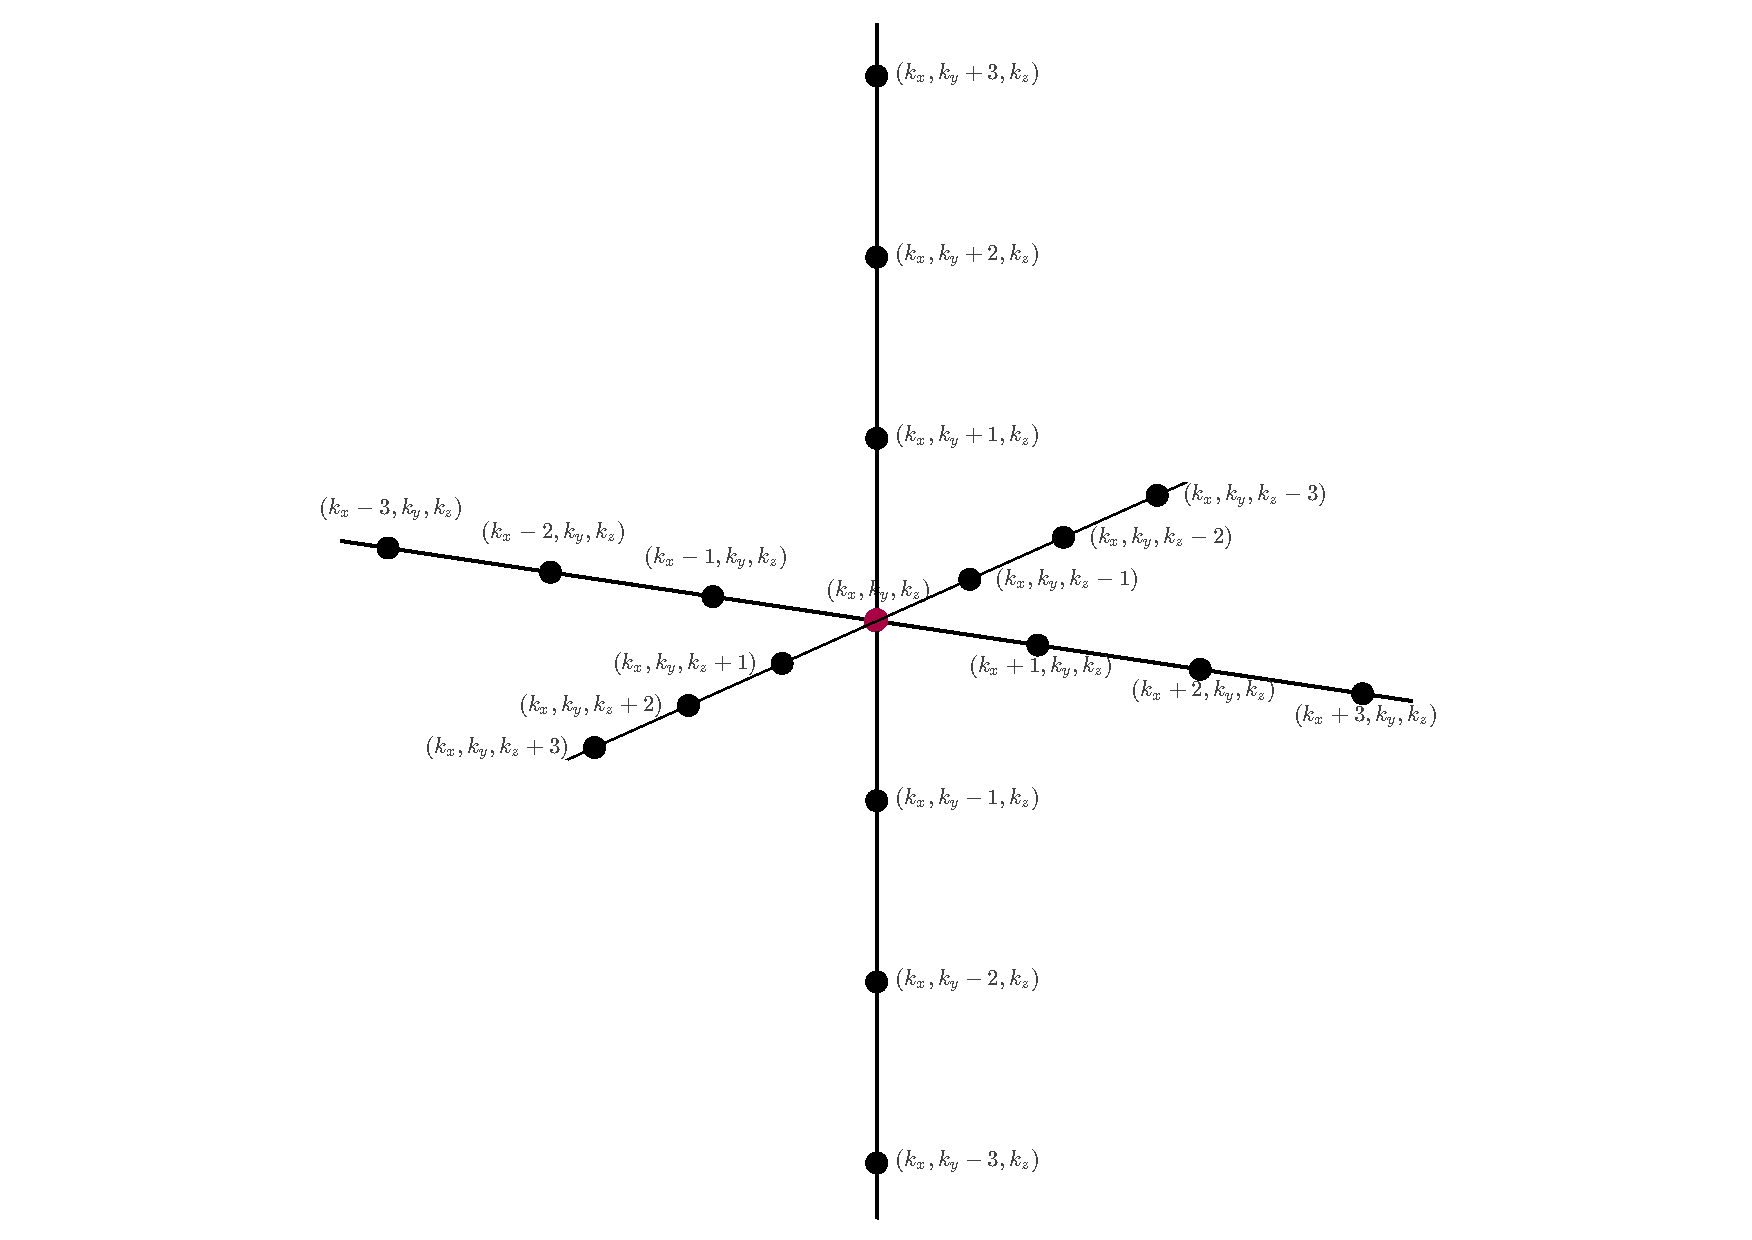
\includegraphics[width=0.9\textwidth]{\localPath/figures/stencil.pdf}
  \caption{Présentation des \emph{stencils} utilisés par la méthode WENO5 pour calculer le flux numérique.}
  \label{fig:intro:stencil}
\end{figure}

La méthode WENO5 consiste en 3 interpolations, sur 3 \emph{stencils} différents, comme l'illustre la figure~\ref{fig:intro:stencil}, pondérées par des poids non-linéaires issus des approximations des dérivées successives de $f$. L'écriture des poids s'effectue comme suit dans le cas $f^-=0$ :
$$
  \begin{aligned}
    \beta_0 &= \frac{13}{12}( \underbrace{f^+_{j-2} - 2f^+_{j-1} + f^+_{j}}_{\Delta x^2(f''_{j} + \mathcal{O}(\Delta x))})^2   + \frac{1}{4}( \underbrace{  f^+_{j-2} - 4f^+_{j-1} + 3f^+_{j}  }_{ 2\Delta x ( f'_{j} + \mathcal{O}(\Delta x^2))})^2 \\
    \beta_1 &= \frac{13}{12}( \underbrace{f^+_{j-1} - 2f^+_{j}   + f^+_{j+1}}_{\Delta x^2(f''_{j} + \mathcal{O}(\Delta x^2))} )^2 + \frac{1}{4}( \underbrace{  f^+_{j-1} -               f^+_{j+1}}_{ 2\Delta x   f'_{j} + \mathcal{O}(\Delta x^2))})^2 \\
    \beta_2 &= \frac{13}{12}( \underbrace{f^+_{j}   - 2f^+_{j+1} + f^+_{j+2}}_{\Delta x^2(f''_{j} + \mathcal{O}(\Delta x))} )^2   + \frac{1}{4}( \underbrace{ 3f^+_{j}   - 4f^+_{j+1} +  f^+_{j+2}}_{-2\Delta x ( f'_{j} + \mathcal{O}(\Delta x^2))})^2 \\
  \end{aligned}
$$
où les coefficients $\beta_0$ sont appelés indicateurs de continuité (\emph{indicators of smoothness}). Ce qui nous permet de calculer les poids définis par :
$$
  \alpha_i = \frac{\gamma_i}{(\varepsilon + \beta_i)^2},\quad i=0,1,2
$$
où $\varepsilon$ est un paramètre numérique pour assurer la non nullité du dénominateur, il sera pris à $10^{-6}$ ; et avec $\gamma_0=\frac{1}{10}$, $\gamma_1=\frac{6}{10}$ et $\gamma_2=\frac{3}{10}$. La normalisation des poids s'effectue comme suit :
$$
  w_i = \frac{\alpha_i}{\sum_m \alpha_m},\quad i=0,1,2
$$
Nous pouvons ensuite calculer les flux numériques pour WENO5 \cite{Shu:2003}, donnés par :
$$
  \begin{aligned}
    \hat{f}_{j+\frac{1}{2}}^+   =\ & w_0\left(  \frac{2}{6}f^+_{j-2} - \frac{7}{6}f^+_{j-1} + \frac{11}{6}f^+_{j}   \right)
                                +    w_1\left( -\frac{1}{6}f^+_{j-1} + \frac{5}{6}f^+_{j}   +  \frac{2}{6}f^+_{j+1} \right) \\
                                +  & w_2\left(  \frac{2}{6}f^+_{j}   + \frac{5}{6}f^+_{j+1} -  \frac{1}{6}f^+_{j+2} \right).
  \end{aligned}
$$
La méthode WENO5 prend la forme finale :
$$
  \partial_xf(x_j) \approx \frac{1}{\Delta x}\left[ \left(\hat{f}_{j+\frac{1}{2}}^+ - \hat{f}_{j-\frac{1}{2}}^+ \right) + \left(\hat{f}_{j+\frac{1}{2}}^- - \hat{f}_{j-\frac{1}{2}}^- \right) \right].
$$

Il existe des variantes de la méthode WENO5, permettant de réduire la perte d'ordre à l'approche d'un choc, à savoir WENO-M (\cite{Henrick:2005}) ou WENO-Z (\cite{Borges:2008}). Ces variations se font sur le calcul des poids non-linéaires. Ainsi la méthode WENO-M utilise une fonction de \emph{mappage} pour équilibrer les poids et est définie par :
$$
  \begin{aligned}
    \alpha_i    &= \frac{\gamma_i}{(\epsilon + \beta_i)^2} \\
    \tilde{w}_i &= \frac{\alpha_i}{\sum_k \alpha_k} \\
    g_i         &= w_i\left( \frac{\gamma_i + \gamma_i^2 - 3w_i\gamma_i + w_i^2}{\gamma_i^2 + w_i(1-2\gamma_i)} \right) \\
    w_i         &= \frac{g_i}{\sum_k g_k}
  \end{aligned}
$$
avec le paramètre $\epsilon = 10^{-4}$. La méthode WENO-Z est quant à elle définie par :
$$
  \begin{aligned}
    \alpha_i &= \gamma_i\left( 1+ \frac{\tau_5}{\epsilon + \beta_i} \right) \\
    w_i      &= \frac{\alpha_i}{\sum_k \alpha_k}
  \end{aligned}
$$
avec les paramètres $\epsilon = 10^{-40}$ et $\tau_5 = \beta_0 - \beta_2$. Cette dernière méthode est celle qui réduit le plus la perte d'ordre à l'approche d'une discontinuité. L'étude approfondie de ces méthodes n'est pas envisagée dans ce travail car les solutions de la physique des plasmas ne présentent pas de discontinuités. Il est à noter que ces méthodes conservent la même linéarisation que le schéma WENO5 classique de Jiang et Shu~\cite{Jiang:1996}, ce qui permet d'y appliquer les résultats de stabilités obtenus dans le chapitre~\ref{chap1}.

Il est possible de monter en ordre en suivant les résultats dans~\cite{Wu:2021}, l'ordre 5 sera considéré comme suffisant dans la suite de ce travail.

L'étude de la stabilité de la méthode WENO5 couplée avec différentes méthodes de type Runge-Kutta pour la résolution en temps a été initiée dans~\cite{Wang:2007} où il a été démontré l'instabilité de la méthode couplée avec la méthode d'Euler explicite, il est nécessaire d'avoir au moins un étage supplémentaire permettant d'assurer la stabilité, ou d'utiliser une méthode d'ordre 3. Des estimations de stabilité et de conditions de stabilité ont par la suite été proposées dans \cite{Motamed:2010,Lunet:2017}. Une étude automatique de la stabilité est présentée dans~\cite{Crouseilles:2019b} qui constitue le chapitre~\ref{chap1} de ce document.

% --------------------------------------------------------------------
\subsection{Méthode semi-lagrangienne}
% --------------------------------------------------------------------

Une méthode très populaire pour la résolution numérique de l'équation de Vlasov est la méthode semi-lagrangienne. Celle-ci s'adapte très bien à notre problème car les termes de transports sont linéaires. Elle a l'avantage de ne pas introduire de contrainte de stabilité. La méthode semi-lagrangienne repose sur la remonté des caractéristique, prenons pour exemple l'équation :
$$
  \partial_t u + a\partial_xu = 0,\quad u(t=0,x)=u_0(x),
$$
ce qui correspond à l'équation~\ref{eq:0:dtudxfu} avec le flux $f$ linéaire par rapport à l'inconnue $u$. On définit les caractérisitique le long desquelles $u$ est constante :
$$
  \begin{cases}
    \dot{x}(s) = a \\
    x(t) = x
  \end{cases}
$$
dont la solution s'écrit $x(s) = a(s-t)+x$. Avec $u(s,x(s))=u(t,x(t))$ on a $u(s,a(s-t)+x) = u(t,x)$ et en prenant $s=t^n=n\Delta t$, et $t=t^{n+1}$, on a :
$$
  u(t^{n+1},x) = u(t^n,x-a\Delta t),\quad \forall x\in[0,L]
$$
Pour connaître $u(t^{n+1},x_j)$ de $u(t^n,\cdot)$, on pose $x=x_j$ : $u(t^{n+1},x_j) = u(t^n,x_j-a\Delta t)$, comme l'illustre la figure~\ref{fig:intro:semilag}. Dans le cadre d'un schéma numérique, $x_j-a\Delta t$ n'étant pas un point de la grille, il faut évaluer en $x_j-a\Delta t$ un polynôme par morceaux, construit à partir des données $u(t^n,x_k)$, $k\in\mathbb{N}$. Plusieurs méthodes d'interpolation sont alors envisageable, la méthode par splines permet une reconstruction gloable de la solution~\cite{Cheng:1976,Sonnendrucker:2015} ; une approche plus locale à partir des données d'un \emph{stencil}, c'est-à-dire des données $u(x_{j^\star-d},t^n)$ jusqu'à $u(x_{j^\star+d},t^n)$, à l'aide d'un polynôme d'interpolation, comme un polynôme de Lagrange de degré $2d+1$, est aussi envisageable~\cite{Charles:2013}. Nous utiliserons cette approche locale avec $d=2$ par la suite.

\begin{figure}[h]
  \centering
  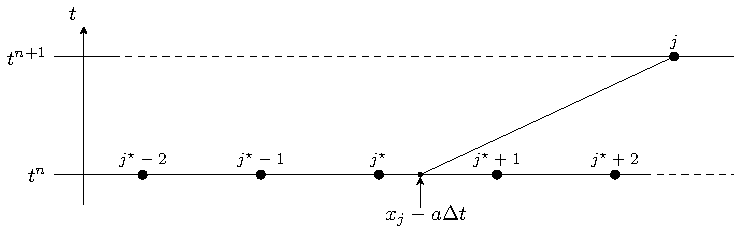
\includegraphics[width=0.9\textwidth]{\localPath/figures/semilag.pdf}
  \caption{Méthode des caractéristiques pour une méthode semi-lagrangienne avec une vitesse de transport $a>0$, et $d=2$.}
  \label{fig:intro:semilag}
\end{figure}


% --------------------------------------------------------------------
\subsection{Méthode pseudo-spectrale}
% --------------------------------------------------------------------

Une autre méthode souvent utilisée pour la résolution d'équations aux dérivées partielles est la méthode pseudo-spectrale qui consiste à approcher les opérateurs différentiels dans l'espace de Fourier à l'aide de transformées de Fourier. Cette méthode permet de transformer une équation aux dérivées partielles en un système d'équations différentielles ordinaires en transformant par exemple une dérivée dans l'espace réel en un produit dans l'espace de Fourier. Nous considèrerons ici la transformée de Fourier discrète, cela consiste à réécrire notre fonction $u$, $L$-périodique et de classe $C^1$, sous la forme :
$$
  u(x) = \sum_{\kappa=-\infty}^{+\infty} \hat{u}_\kappa e^{i\frac{2\pi \kappa}{L}x},
$$
où les coefficients de Fourier $\hat{u}_\kappa$ sont définis par :
$$
  \hat{u}_\kappa = \frac{1}{L}\int_0^L u(x)e^{-i\frac{2\pi \kappa}{L}x}\dd{x}.
$$

En n'ayant la connaissance de la fonction $u$ qu'en des points $x_j = j\frac{L}{N}$, $j=0,\dots,N-1$ de la grille, il est possible d'approcher les coefficient de Fourier par une somme discrète :
$$
  \hat{u}_\kappa \approx \frac{1}{N-1}\sum_{j=0}^N u(x_j) e^{=i\frac{2\pi j}{N}\kappa}.
$$

Transformer une dérivée en un produit nous sera utile au long de ce travail dans deux contextes, un premier linéaire :
$$
  \partial_t u + a\partial_x u = 0,\qquad u(t=0,x)=u_0(x)
$$
devenant après une transformée de Fourier : $\partial_t \hat{u}_\kappa + ai\kappa \hat{u}_\kappa = 0$ et pouvant se résoudre exactement en temps : $\hat{u}_\kappa(t) = \exp(-ia\kappa t)\hat{u}_\kappa(0)$. Cela correspond à la partie linéaire d'une méthode de Lawson~\ref{ssec:0:lawson}. L'autre cas d'utilisation sera pour un terme non-linéaire de la forme :
$$
  \partial_t u + \partial_xf(u) = 0,\qquad u(t=0,x)=u_0(x)
$$
devenant alors après une transformée de Fourier : $\partial_t\hat{u}_\kappa + i\kappa\widehat{\left(f(u)\right)}_\kappa = 0$. Ce terme n'ayant pas de solution explicite il sera résolu numériquement pas une méthode Runge-Kutta, correspondant au terme non-linéaire d'une méthode de Lawson.

Nous utiliserons l'algorithme de transformée de Fourier rapide (\emph{fast Fourier transform} ou FFT) pour effectuer numériquement cette opération, dont une implémentation est proposée dans~\cite{Saramito:2013}. Cet algorithme possède une complexité en temps de $\order{N\log N}$, où $N$ est le nombre de points de discrétisation en espace.


% annexe
\begin{subappendices}
\section{Dérivation du modèle de Vlasov-Maxwell hybride linéarisé}

\subsection{Dérivation du modèle de Vlasov-Maxwell hybride}
\label{ssec:0:vmh}

On s'intéresse ici à démontrer la proposition~\ref{pro:0:vmh}.
\begin{proof}
  Pour écrire le modèle hybride, on distingue deux populations de particles dans le modèle de Vlasov-Maxwell~\eqref{eq:0:vlasov}-\eqref{eq:0:poisson}, une population de particules froides $f_c$ donc la vitesse thermique est faible, et une seconde population de particules chaudes $f_h$ dont la vitesse thermique est grande. Ces populations sont supposées indépendantes, l'équation de Vlasov devient :
  $$
    \begin{aligned}
      \pdv{f_c}{t} &+ \vb{v}\cdot\nabla_{\vb{x}} f_c + \frac{q_e}{m_e}\left( \vb{E} + \vb{v}\times(\vb{B}+\vb{B}_0) \right)\cdot\nabla_{\vb{v}} f_c = 0 \\
      \pdv{f_h}{t} &+ \vb{v}\cdot\nabla_{\vb{x}} f_h + \frac{q_e}{m_e}\left( \vb{E} + \vb{v}\times(\vb{B}+\vb{B}_0) \right)\cdot\nabla_{\vb{v}} f_h = 0
    \end{aligned}
  $$
  et l'équation de Maxwell-Ampère~\eqref{eq:0:maxwellE} et de Maxwell-Gauss~\eqref{eq:0:poisson} deviennent :
  $$
    \begin{aligned}
      \frac{1}{c^2}\pdv{\vb{E}}{t} &= \nabla_{\vb{x}}\times \vb{B} - \mu q_e\int \vb{v} f_c\dd{\vb{v}} - \mu q_e\int \vb{v} f_h\dd{\vb{v}} \\
      \nabla_{\vb{x}}\cdot\vb{E} &= \frac{1}{\varepsilon_0}\left( q_i\rho_i + q_e\int f_c\dd{\vb{v}} + q_e\int f_h\dd{\vb{v}} \right)
    \end{aligned}
  $$
  On introduit la densité $\rho_c=\rho_c(t,\vb{x})$ et la vitesse moyenne $\vb{u}_c=\vb{u}_c(t,\vb{x})$ des particules froides :
  $$
    \begin{pmatrix}
      \rho_c \\
      \rho_c \vb{u}_c
    \end{pmatrix}
    =
    \int_{\mathbb{R}^3} \begin{pmatrix}
      1 \\
      \vb{v}
    \end{pmatrix} f_c\dd{\vb{v}}
  $$
  Maintenant on calcule les moments de l'équation de Vlasov sur les particules chaudes, c'est-à-dire que l'on multiplie l'équation par $(1,\vb{v})^\top$ puis on intègre en $\vb{v}$ :
  $$
    \begin{aligned}
    \partial_t\int_{\mathbb{R}^3} \begin{pmatrix}
      1 \\
      \vb{v}
    \end{pmatrix}f_c
    &+
    \int_{\mathbb{R}^3}\begin{pmatrix}
      1 \\
      \vb{v}
    \end{pmatrix}(\vb{v}\cdot\nabla_{\vb{x}}f_c)\dd{\vb{v}} \\
    &+
    \frac{q_e}{m_e}\int_{\mathbb{R}^3}\begin{pmatrix}
      1 \\
      \vb{v}
    \end{pmatrix} (\vb{E}\cdot\nabla_{\vb{v}}f_c)\dd{\vb{v}}
    +
    \frac{q_e}{m_e}\int_{\mathbb{R}^3}\begin{pmatrix}
      1 \\
      \vb{v}
    \end{pmatrix}(\vb{v}\times(\vb{B}+\vb{B}_0) \cdot\nabla_{\vb{v}}f_c)\dd{\vb{v}}
    = 0.
    \end{aligned}
  $$
  On réécrit cela comme deux équations, une par moment calculé :
  $$
    \begin{aligned}
      &\partial_t\rho_c + \nabla_{\vb{x}}\cdot(\rho_c\vb{u}_c) = 0 \\
      &\partial_t\rho_c\vb{u}_c + \int\vb{v}(\vb{v}\cdot\nabla_{\vb{x}}f_c)\dd{\vb{v}} + \frac{q_e}{m_e}\int\vb{v}(\vb{E}\cdot\nabla_{\vb{v}}f_c)\dd{\vb{v}} \\
      &\phantom{\partial_t\rho_c\vb{u}_c + \int\vb{v}(\vb{v}\cdot\nabla_{\vb{x}}f_c)\dd{\vb{v}}}
        + \frac{q_e}{m_e}\int\vb{v}\left((\vb{v}\times(\vb{B}+\vb{B}_0))\cdot\nabla_{\vb{v}}f_c\right)\dd{\vb{v}} = 0
    \end{aligned}
  $$
  Cette deuxième équation contient plusieurs termes que l'on peut traiter individuellement en les regardant par composante :
  $$
    \begin{aligned}
      \left( \int\vb{v}(\vb{v}\cdot\nabla_{\vb{x}}f_c)\dd{\vb{v}} \right)_i
          &= \int v_i \sum_{j=1}^3v_j\partial_{x_j}f_c\dd{v_i} \\
          &= \sum_{j=1}^3\partial_{x_j}\int v_iv_jf_x\dd{v_i} \\
          &= \sum_{j=1}^3\partial_{x_j}\int (\vb{v}\otimes\vb{v})_{ij}f_x\dd{v_i} \\
          &= \left( \nabla_{\vb{x}}\cdot\int \vb{v}\otimes\vb{v} f_c\dd{\vb{v}} \right)_i \\
          &= \left( \nabla_{\vb{x}}\cdot(\rho_c\vb{u}_c\otimes\vb{u}_c) \right)_i
    \end{aligned}
  $$
  où on note $\otimes$ le produit tensoriel : $(\alpha\otimes\beta)_{i,j} = \alpha_i\beta_j$. Le terme suivant :
  $$
    \begin{aligned}
      \left( \frac{q_e}{m_e}\int\vb{v}(\vb{E}\cdot\nabla_{\vb{v}}f_c)\dd{\vb{v}} \right)_i
          &= \frac{q_e}{m_e}\int v_i\sum_{j=1}^3 E_j\partial_{v_j}f_c\dd{v_i} \\
          &= -\frac{q_e}{m_e}\sum_{j=1}^3 e_j\int\partial_{v_j}(v_i)f_c\dd{v_i} \\
          &= -\frac{q_e}{m_e}E_i\int f_c\dd{v_i} \\
          &= -\frac{q_e}{m_e}(\rho_c E)_i.
    \end{aligned}
  $$
  Et enfin le troisième terme :
  $$
    \begin{aligned}
      \left( \frac{q_e}{m_e}\int\vb{v}\left((\vb{v}\times(\vb{B}+\vb{B}_0))\cdot\nabla_{\vb{v}}f_c\right)\dd{\vb{v}} \right)_i
          &= \frac{q_e}{m_e}\int v_i\sum_{j=1}^3\left(\vb{v}\times(\vb{B}+\vb{B}_0)\right)_j\partial_{v_j}f_c\dd{v_i} \\
          &= -\frac{q_e}{m_e}\sum_{j=1}^3\int\partial_{v_j}(v_i)\left(\vb{v}\times(\vb{B}+\vb{B}_0)\right)_jf_c\dd{v_i} \\
          &= -\frac{q_e}{m_e}\int\left(\vb{v}\times(\vb{B}+\vb{B}_0)\right)_i f_c\dd{v_i} \\
          &= \left[ -\frac{q_e}{m_e}\left(\int\vb{v}f_c\dd{\vb{v}}\right)\times(\vb{B}+\vb{B}_0) \right]_i \\
          &= \left[ -\frac{q_e}{m_e}(\rho_c\vb{u}_c)\times(\vb{B}+\vb{B}_0) \right]_i.
    \end{aligned}
  $$
  On peut ainsi réécrire les moments comme :
  $$
    \begin{aligned}
      \partial_t\rho_c + \nabla_{\vb{x}}\cdot(\rho_c\vb{u}_c) &= 0 \\
      \partial_t(\rho_c\vb{u}_c) + \nabla_{\vb{x}}\cdot(\rho_c\vb{u}_c\otimes\vb{u}_c) - \frac{q}{m}\left( \rho_c\vb{E} + (\rho_c\vb{u}_c)\times(\vb{B}+\vb{B}_0) \right) &=0.
    \end{aligned}
  $$

  On définit maintenant le courant induit par les particules froides $\vb{j}_c=\vb{j}_c(t,\vb{x})$ comme étant une renormalisation du courant $\rho_c\vb{u}_c$ :
  $$
    \vb{j}_c = q_e(\rho_c\vb{u}_c)
  $$
  ce qui nous permet de réécrire l'équation du deuxième moment de $f_c$ comme :
  $$
    \partial_t\vb{j}_c + \nabla_{\vb{x}}\cdot\frac{\vb{j}_c\otimes\vb{j}_c}{q_e\rho_c} = \frac{q_e}{m_e}\left( q_e\rho_c\vb{E} + \vb{j}_c\times(\vb{B}+\vb{B}_0) \right)
  $$

  On écrit ainsi les équations de Vlasov-Maxwell hybride :
  \begin{align}
      \partial_t f_h &+ \vb{v}\cdot\nabla_{\vb{x}} f_h + \frac{q_e}{m_e}\left( \vb{E} + \vb{v}\times(\vb{B}+\vb{B}_0) \right)\cdot\nabla_{\vb{v}} f_h = 0 \\
      \partial_t\rho_c &+ \frac{1}{q_e}\nabla_{\vb{x}}\cdot(\vb{j}_c) = 0 \\
      \partial_t\vb{j}_c &+ \nabla_{\vb{x}}\cdot\frac{\vb{j}_c\otimes\vb{j}_c}{q_e\rho_c} - \frac{q_e}{m}\left( q_e\rho_c\vb{E} + \vb{j}_c\times(\vb{B}+\vb{B}_0) \right) = 0 \\
      \pdv{\vb{B}}{t} &= - \nabla_{\vb{x}}\times\vb{E} \\
      \frac{1}{c^2}\partial_t\vb{E} &= \nabla_{\vb{x}}\times \vb{B} - \mu\vb{j}_c - \mu q_e\int \vb{v} f_h\dd{\vb{v}} \\
      \nabla_{\vb{x}}\cdot\vb{E} &= \frac{1}{\varepsilon_0}\left( q_i\rho_i + q_e\rho_c + q_e\int f_h\dd{\vb{v}} \right)
  \end{align}
\end{proof}

\subsection{Dérivation du modèle de Vlasov-Maxwell hybride linéarisé}
\label{ssec:0:vmhl}

On s'intéresse ici à démontrer la proposition~\ref{pro:0:vmhl}.
\begin{proof}
  On souhaite linéariser le système~\eqref{eq:0:vmh:1}-\eqref{eq:0:vmh:6} autour de l'état d'équilibre $\left(\rho_c^{(0)},0,0,0,f_h^{(0)}(\vb{v})\right)$, avec $f_h^{(0)}(\vb{v})$ une fonction telle que $\int\vb{v}f_h^{(0)}\dd{\vb{v}} = 0$. En réutilisant la réécriture des inconnues~\eqref{eq:0:linear}, on peut réécrire le système~\eqref{eq:0:vmh:1}-\eqref{eq:0:vmh:6} sous la forme :
  \begin{align}
    \label{eq:0:vmhleps:1}
      \partial_t f_h &+ \vb{v}\cdot\nabla_{\vb{x}} f_h + \frac{q_e}{m_e}\left( \vb{E} + \vb{v}\times(\vb{B}+\vb{B}_0) \right)\cdot\nabla_{\vb{v}} f_h = 0 \\
    \label{eq:0:vmhleps:2}
      \varepsilon\partial_t\rho_c^{(1)} &+ \frac{\varepsilon}{q_e}\nabla_{\vb{x}}\cdot(\vb{j}_c^{(1)}) = 0 \\
    \label{eq:0:vmhleps:3}
      \varepsilon\partial_t\vb{j}_c^{(1)} &+ \varepsilon^2\nabla_{\vb{x}}\cdot\frac{\vb{j}_c^{(1)}\otimes\vb{j}_c^{(1)}}{q_e(\rho_c^{(0)}+\varepsilon\rho_c^{(1)})} - \frac{q_e}{m_e}\left( q_e(\rho_c^{(0)}+\varepsilon\rho_c^{(1)})\varepsilon\vb{E} + \varepsilon\vb{j}_c^{(1)}\times(\varepsilon\vb{B}^{(1)}+\vb{B}_0) \right) = 0 \\
    \label{eq:0:vmhleps:4}
      \varepsilon\partial_t\vb{B}^{(1)} &= - \varepsilon\nabla_{\vb{x}}\times\vb{E}^{(1)} \\
    \label{eq:0:vmhleps:5}
      \frac{\varepsilon}{c^2}\partial_t\vb{E}^{(1)} &= \varepsilon\nabla_{\vb{x}}\times \vb{B}^{(1)} - \varepsilon\mu\vb{j}_c^{(1)} - \varepsilon\mu q_e\int \vb{v} f_h^{(1)}\dd{\vb{v}} \\
    \label{eq:0:vmhleps:6}
      \varepsilon\nabla_{\vb{x}}\cdot\vb{E}^{(1)} &= \frac{1}{\varepsilon_0}\left( q_i\rho_i + q_e\rho_c + q_e\int f_h\dd{\vb{v}} \right)
  \end{align}
  Nous souhaitons négliger les termes non-linéaires d'ordre $\order{\varepsilon^2}$. Dans le système~\eqref{eq:0:vmhleps:1}-\eqref{eq:0:vmhleps:5} On remarque alors que~\eqref{eq:0:vmhleps:2} est la seule équation faisant intervenir $\rho_c^{(1)}$, et cette variable peut être recalculer à partir de~\eqref{eq:0:vmhleps:6} si besoin. L'équation~\eqref{eq:0:vmhleps:2} pourra donc être omise du système par la suite. Par abus de notation, pour la lisibilité, on retirera les indices de variables linéarisées lorsqu'il n'y a pas d'ambiguïté, par conséquent les variables $\vb{j}_c$, $\vb{E}$, $\vb{B}$ qui apparaissent par la suite, donc d'ordre $\varepsilon$ et correspondent à leurs perturbations par rapport à un équilibre nul. On introduit aussi la fréquence de plasma des particules froides $\Omega_{pe}^2 = \frac{q^2\rho_c^{(0)}}{\varepsilon_0m_e}$. On peut alors réécrire le système~\eqref{eq:0:vmhleps:1}-\eqref{eq:0:vmhleps:5} comme :
  \begin{align}
      \partial_t f_h &+ \vb{v}\cdot\nabla_{\vb{x}} f_h + \frac{q_e}{m_e}\left( \vb{E} + \vb{v}\times(\vb{B}+\vb{B}_0) \right)\cdot\nabla_{\vb{v}} f_h = 0 \\
      \partial_t j_c &= \varepsilon_0\Omega_{pe}^2\vb{E} + \frac{q}{m_e}\vb{j}_c\times\vb{B}_0 \\
      \partial_t\vb{B} &= -\nabla_{\vb{x}}\times\vb{E} \\
      \frac{1}{c^2}\partial_t\vb{E} &= \nabla_{\vb{x}}\times\vb{B} - \mu_0\vb{j}_c - \mu_0q_e\int\vb{v}f_h\dd{\vb{v}}
  \end{align}
\end{proof}

\Josselin{Est-ce qu'on ajoute ici l'adimensionnement du système~\eqref{eq:0:vmhl:1}-\eqref{eq:0:vmhl:4} ou un lien vers l'annexe où cela sera fait ?}



\end{subappendices}
